\PassOptionsToPackage{svgnames}{xcolor}
\documentclass[12pt]{article}



\usepackage[margin=0.1in]{geometry}  
\usepackage{graphicx}             
\usepackage{amsmath}              
\usepackage{amsfonts}              
\usepackage{framed}               
\usepackage{amssymb}
\usepackage{array}
\usepackage{amsthm}
\usepackage[nottoc]{tocbibind}
\usepackage{bm}
\usepackage{algorithm}
\usepackage[noend]{algpseudocode}
\usepackage{enumitem}
\usepackage{wrapfig}
\usepackage{titlesec}
\titlespacing*{\section}{0pt}{0.1\baselineskip}{0.1\baselineskip}
\algdef{SE}[SUBALG]{Indent}{EndIndent}{}{\algorithmicend\ }%
\algtext*{Indent}
\algtext*{EndIndent}
  \newcommand\norm[1]{\left\lVert#1\right\rVert}
  \newcommand\TCP{\texttt{TCP} }
  \newcommand\UDP{\texttt{UDP} }
  \newcommand\IP{\texttt{IP} }
  \newcommand\PrivK{\mathrm{PrivK}}
  \newcommand\MacForge{\mathrm{Mac-Forge}}
  \newcommand\MacSForge{\mathrm{Mac-sForge}}
\setlength{\parindent}{0cm}
\setlength{\parskip}{0em}
\newcommand{\Lim}[1]{\raisebox{0.5ex}{\scalebox{0.8}{$\displaystyle \lim_{#1}\;$}}}
\newtheorem{definition}{Definition}[section]
\newtheorem{theorem}{Theorem}[section]
\newtheorem{notation}{Notation}[section]
\theoremstyle{definition}
\setcounter{tocdepth}{1}
\setcounter{section}{0}
\begin{document}
\title{Revision notes - CS4236}
\author{Ma Hongqiang}
\maketitle
\tableofcontents


\twocolumn
\section{Classical Cipher System}
\begin{definition}[Syntax of Encryption]
\hfill\\\normalfont 
\begin{itemize}
\item $\mathcal{M}$: Message space, which a set of legal messages
\item \texttt{Gen}: Procedure for generating key. It should be a probabilistic algorithm that outputs a key $k\in K$ chosen according to some distribution.
\item \texttt{Enc}: Procedure for encrypting. Takes as input a key $k$ and message $m$ and outputs a ciphertext $c$. Denote by $\texttt{Enc}_k(m)$.
\item \texttt{Dec}: Procedure for decrypting. Takes as input a key $k$ and a ciphertext $c$ and outputs a plaintext $m$. Denote by $\texttt{Dec}_k(c)$.
\end{itemize}
\end{definition}
\begin{theorem}[Correctness Requirement]
\hfill\\\normalfont An encryption scheme must satisfy the correctness requirement: \\
\fbox{For every key $k$ output by \texttt{Gen} and every message $m\in\mathcal{M}$, we have $\texttt{Dec}_k(\texttt{Enc}_k(m))=m$
}
\end{theorem}
\begin{theorem}[Kerckhoff's Principle]
\hfill\\\normalfont Security should rely \textit{only} on the secrecy of the key.
\end{theorem}
Therefore, there should never be ``security by obsecurity''.
\subsection{Principles of Modern Cryptography}
\begin{definition}[Security Definition]
\hfill\\\normalfont Security Definition is a tuple
\begin{enumerate}
  \item \textbf{Security guarantee}: what the scheme is intended to prevent the attack from doing; and
  \item \textbf{Threat model}: the capability of the adversary
\end{enumerate}
Typically, the security guarantee is to make it impossible for an attacker to \textbf{learn any additional information} aboue the underlying plaintext, whereas the threat model can be either one of the below:
\begin{itemize}
  \item Ciphertext-only attack: most basic attack
  \item Known-plaintext attack: attacker learns plaintext/cipphertext pairs
  \item Chosen-plaintext-attack: attacker obtains plaintext/ciphertext pairs for plaintext of its choice
  \item Chosen-ciphertext attack: attacker obtains plaintext/ciphertext pairs for ciphertexts of its choice
\end{itemize}
\end{definition}
\subsection{Perfectly Secret Encryption}
There are two equivalent definition of perfect secrecy.
\begin{definition}[Perfect Secrecy]
\hfill\\\normalfont An encryption scheme(\texttt{Gen}, \texttt{Enc},\texttt{Dec}) with message space $\mathcal{M}$ is \textbf{perfectly secret} if for \textit{every} probability distribution over $\mathcal{M}$, every message $m\in \mathcal{M}$, and every ciphertext $c\in \mathcal{C}$ for which $P(C=c)>0$, we have
$
P(\mathcal{M}=m|\mathcal{C}=c) = P(\mathcal{M}=m)
$
\end{definition}
\begin{definition}[Perfect Secrecy Equivalent Definition]
\hfill\\\normalfont For every $m, m'\in\mathcal{M}$, and every $c\in\mathcal{C}$, we have
$
P(\texttt{Enc}_K(m)=c) = P(\texttt{Enc}_K(m') = c)
$
The equivalency can be derived by using the lemma below
$
P(\mathcal{C}=c\mid \mathcal{M}=m) = P(\mathcal{C}=c)
$
is equivalent to the perfect secrecy definition.
\end{definition}
\begin{definition}[Perfect Indistinguishability]
\hfill\\\normalfont Consider an experiment with an adversary $\mathcal{A}$ and an encryption oracle $\Pi=(\texttt{Gen}, \texttt{Enc},\texttt{Dec})$. The process goes like this:
\begin{enumerate}
  \item $\mathcal{A}$ sends $m_0, m_1\in\mathcal{M}$ to $\Pi$
  \item $\Pi$ generates key $k$ using \texttt{Gen}; picks $0$ or $1$ with equal chance and set as $b$; send back $\texttt{Enc}_k(m_b)$.
  \item $\mathcal{A}$ outputs the guess of $b$ as $b'$.
\end{enumerate}
We say that $\Pi$ is perfectly indistinguishable if for \textit{every} $\mathcal{A}$, it holds that
$
P(b'=b) = \frac{1}{2}
$
\end{definition}
It is known that perfect indistinguishability is equivalent to perfect secrecy.




\section{Computational Secrecy}
The perfect secrecy is unnecessarily strong, and therefore we relax the constraint from unlimited computational power and perfect indistinguishability to efficient computational power, and a weaker version of indistinguishability, called computational indistinguishability.
\begin{definition}[Computationally {$(t,\epsilon)$}-indistinguishable]
\hfill\\\normalfont Encryption scheme $\Pi=(\texttt{Gen},\texttt{Enc},\texttt{Dec})$ is $(t,\epsilon)$-indistinguishable if for every $\mathcal{A}$ running in time at most $t$, it holds that
$
P(\PrivK _{\mathcal{A},\Pi}^{eav} = 1) \leq \frac{1}{2}+\epsilon
$
\end{definition}
The choice of $t$ and $\epsilon$ is troublesome. We can define computational indistinguishability in \textit{asymptotic} approach.
\begin{definition}[Asymptotically Secure]
\hfill\\\normalfont A scheme is secure if any \textbf{probabilistic polynomial-time}(PPT) adversary succeeds in breaking the scheme with at most \textbf{negligible probability}.\\
Here, an algorithm $A$ runs in polynomial time, if there exists a polynomial $p$ such that for every input $x\in \{0,1\}^\ast$, the computation of $A(x)$ terminates within at most $p(|x|)$ steps. An algorithm is probabilistic, if it can access an unbiased random bit at each step.\\
A function is negligible if for every positive polynomial $p$, there is an $N$, such that for all integer $n>N$, it holds that $f(n)<\frac{1}{p(n)}$.
\end{definition}
\textbf{Remark}: 
\begin{itemize} 
  \item suppose $f,g$ is negligible, and $p$ polynomial, then $f+g$ and $f\times p$ are both negligible.
  \item Both the running time and the probability can be parameterised by a single variable $n$, which is typically the key length.
\end{itemize}
\subsection{Security for Encryption}
Before we define the security for encryption, we first define private key encryption scheme.
\begin{definition}[Private Key Encryption]
\hfill\\\normalfont A private-key encryption scheme is a PPT algorithm $\Pi=(\texttt{Gen},\texttt{Enc},\texttt{Dec})$ such that
\begin{itemize}
  \item \texttt{Gen} outputs a key $k$ with length $n$.
  \item \texttt{Enc} takes as input a key $k$ and a plaintext message $m\in\{0,1\}^\ast$, and outputs a ciphertext $c=\texttt{Enc}_k(m)$.
  \item \texttt{Dec} takes as input a key $k$ and a ciphertext $c$, and outputs a message $m=\texttt{Dec}_k(c)$.
\end{itemize}
\end{definition}
We then define what we called, semantic security.
\begin{definition}[Semantic Security]
\hfill\\\normalfont A private key encryption scheme $\Pi$ is \textbf{semantically secure in the presense of an eavesdropper} if any probabilistic polynomial time algorithm $\mathcal{A}$ are infeasible to learn any partial information about the plaintext from the ciphertext. 
\end{definition}
The exact definition is mathematically complex and is not stated here. However, this definition of semantic security is equivalent to the indistinguishable encryption in the presense of an eavesdropper, whose definition is given below:
\begin{definition}[Indistinguishable Encryption]
\hfill\\\normalfont A private-key encryption scheme $\Pi$ has \textbf{indistinguishable encryptions in the presence of an eavesdropper} if for all probabilistic polynomial-time adversaries $\mathcal{A}$, there exists a negligible function $\mathbf{negl}$ such that
$
P(\PrivK _{\mathcal{A},\Pi}^\text{eav}(n))\leq \frac{1}{2}+\mathbf{negl}(n)
$
for all $n$, where $n$ is the security parameter.
\end{definition}
Note that the experiment now takes in $n$, which is used to generate the random key $k$.\\
We then introduce an equivalent definition as the above, which is used later in some proof.
\begin{definition}[Equivalent Indistinguishable Encryption]
\hfill\\\normalfont Define $\PrivK _{\mathcal{A},\Pi}^\text{eav}(n,b)$ to be the same as above, except that the fixed bit $b$ is used, rather than being chosen by $\Pi$ at random. In addition, denote the output bit $b'$ from $\mathcal{A}$ in $\PrivK _{\mathcal{A},\Pi}^\text{eav}(n,b)$ by $\text{output}(\PrivK _{\mathcal{A},\Pi}^\text{eav}(n,b))$. The following definition essentially states that $\mathcal{A}$ cannot determine whether it is running in experiment $\PrivK _{\mathcal{A},\Pi}^\text{eav}(n,0)$ or $\PrivK _{\mathcal{A},\Pi}^\text{eav}(n,1)$.\\

A private key encryption scheme $\Pi$ has indistinguishable encryption in the presence of eavesdropper if for all probabilistic polynomial-time adversaries $\mathcal{A}$, there exists a negligible function $\mathbf{negl}$ such that
$
|P(\text{output}(\PrivK _{\mathcal{A},\Pi}^\text{eav}(n,0))=1)-P(\text{output}(\PrivK _{\mathcal{A},\Pi}^\text{eav}(n,1))=1)|\leq \mathbf{negl}(n)
$
\end{definition}
\subsection{Pseudorandom Generators(PRG)}
\begin{definition}[Pseudorandom Generator]
\hfill\\\normalfont Let $l(\cdot)$ be a polynomial and let $G$ be a deterministic polynomial-time algorithm such that upon any input $s\in\{0,1\}^n$, algorithm $G$ outputs a string of length $l(n)$.\\

We say that $G$ is a \textbf{pseudorandom generator} if
\begin{enumerate}
 \item \textbf{Expansion}: For every $n$, it holds that $l(n)>n$.
 \item \textbf{Pseudorandomness}: For all probabilistic polynomial-time(PPT) distinguishers $D$, there exists a negligible function $\mathbf{negl}$ such that
 $
|P(D(r)=1)-P(D(G(s))=1)|\leq \mathbf{negl}(n)
 $
where $r$ is chosen uniformly at random from $\{0,1\}^{l(n)}$, the seed $s$ is chosen uniformly at random from $\{0,1\}^n$.
\end{enumerate}
Here, $l$ is the expansion factor of $G$.
\end{definition}
With PRG, we construct an encryption scheme that has indistinguishable encryptions in the presence of an eavesdropper. 
\begin{definition}[Construction]
\hfill\\\normalfont Let $G$ be a pseudorandom generator with expansion factor $l$. Define a private-key encryption scheme for messages of legnth $l$ as follows:
\begin{itemize}
  \item $\texttt{Gen}$: on input of $n$, choose $k\leftarrow \{0,1\}^n$ uniformly at random and output it as the key
  \item $\texttt{Enc}$: on input a key $k\in\{0,1\}^n$ and a message $m\in\{0,1\}A^{l(n)}$, output the ciphertext
  $
c:=G(k)\oplus m
  $
  \item $\texttt{Dec}$: on input a key $k\in\{0,1\}^n$ and a ciphertext $c\in\{0,1\}^{l(n)}$, output the plaintext message
$
m:=G(k)\oplus c
$
\end{itemize}
\end{definition}
We claim the above construction has indistinguishable encryption in presence of eavesdropper.\\
\textbf{Proof}
Suppose there is a PPT $\mathcal{A}$ such that it violates the definition of indistinguishable encryption, then we can construct a PPT that distinguishes the output of $G$ from a truly random string. \\
Let $\mathcal{A}$ be a PPT adversary, and define $\varepsilon$ as
$
\varepsilon(n):=P[\PrivK _{\mathcal{A},\Pi}^\text{eav}(n)=1]-\frac{1}{2}
$
We use $\mathcal{A}$ to construct a distinguisher $D$ for pseudorandom generator $G$, such that $D$ can also succeed with probability $\epsilon(n)$.\\
The distinguisher is given a string $w$ as input, and it is to determine whether $w$ is chosen uniformly at random, or whether $w$ is generated by choosing a random $k$ and computing $w:=G(k)$. $D$ emulates the eavesdropping experiment for $\mathcal{A}$ and observes whether $\mathcal{A}$ succeeds or not. If $\mathcal{A}$ succeeds then $D$ guesses that $w$ must have been a pseudorandom string, while if $\mathcal{A}$ does not succeed then $D$ guesses $w$ is a random string. In detail:
\begin{itemize}
  \item[] \textbf{Distinguisher} $D$:
  \item[] $D$ is given as input a string $w\in\{0,1\}^{l(n)}$.
  \item[1.] Run $\mathcal{A}$ to obtain the pair of messages $m_0,m_1\in\{0,1\}^{l(n)}$.
  \item[2.] Choose a random bit $b\leftarrow\{0,1\}$. Set $c:=w\oplus m_b$.
  \item[3.] Give $c$ to $\mathcal{A}$ and obtain output $b'$. In a sense, we output $1$ if $b'=b$ and $0$ otherwise.
\end{itemize}
We also, define a modified encryption scheme $\tilde{\Pi}$ that is exactly one-time pad encryption, i.e. \texttt{Gen} can output a completely random key $k$ of length $l(n)$. By perfect secrecy of one-time pad, we have
$
P[\PrivK _{\mathcal{A},\Pi}^\text{eav}(n)=1]=\frac{1}{2}
$
The main observations are:
\begin{enumerate}
  \item If $w$ is chosedn uniformly at random from $\{0,1\}^{l(n)}$, then the view of $\mathcal{A}$ when run as a subroutine by the distinguisher $D$ is distributed identically to the view of $\mathcal{A}$ in teh experiment $\PrivK _{\mathcal{A},\tilde{\Pi}}^\text{eav}(n)$. This is because $\mathcal{A}$ is given a ciphertext $c=w\oplus m_b$ where $w$ is completely random.
  \item On the other hand, if $w=G(k)$, where $k\leftarrow\{0,1\}^n$ is chosen uniformly at random, the the view of $\mathcal{A}$ when run as a subroutine by $D$ is distributed identically to the view of $\mathcal{A}$ in experiment $\PrivK _{\mathcal{A},\Pi}^\text{eav}(n)$. This is because $\mathcal{A}$ is given a ciphertext $c=w\oplus m_b$ where $w=G(k)$ for a uniformly distributed value $k\in \{0,1\}^n$.
\end{enumerate}
Therefore, if $w$ is chosen uniformly at random 
$
P(D(w)=1)=\frac{1}{2}
$
In contrast, when $w=G(k)$, we have
$
P(D(w))=P(D(G(k)))=\frac{1}{2}+\varepsilon(n)
$
Therefore, 
$
|P(D(w)=1)-P(D(G(k))=1)|=\varepsilon(n)
$
where $w$ is randomly chosen in $\{0,1\}^{l(n)}$ and $k$ randomly chosen in $\{0,1\}^{n}$. Since $G$ is a pseudorandom generator, $\varepsilon$ must be negligible by its definition.  

\section{CPA Security}
Our definition of $\PrivK _{\mathcal{A},\Pi}^\text{eav}$, although can be used to prove the security of encryption, has several limitations:
\begin{itemize}
  \item It only considers ciphertext-only attacks, whereas \textit{real} attackers may have more capabilities
  \item It only considers single ciphertext observation, whereas \textit{real} attackers may observe more than one ciphertext
\end{itemize}
From this section onwards, we give more capabilities to adversary.
\begin{definition}[Chosen Plaintext Attack]
\hfill\\\normalfont \textbf{Chosen Plaintext Attack} is an attack in which adversary can influence the sender to encrypt message $m_1,\ldots$ with the \textit{same} unknown key $k$ and observe the corresponding ciphertext $c_1,\ldots$.
\end{definition}
\begin{definition}[CPA Security]
\hfill\\\normalfont Experiment $\PrivK_{\mathcal{A},\Pi}^\text{cpa}$ for encryption scheme $\Pi$ and adversary $\mathcal{A}$ is defined as below:
\begin{itemize}
  \item $k\leftarrow \texttt{Gen}(1^n)$.
  \item $\mathcal{A}$ interacts with $\texttt{Enc}_k()$.
  \item $\mathcal{A}$ outputs $m_0, m_1$. Oracle calculates $b$ randomly chosen from $\{0,1\}$ and sends $c\leftarrow \texttt{Enc}_k(m_b)$.
  \item $\mathcal{A}$ continues interacting with $\texttt{Enc}_k()$.
  \item $\mathcal{A}$ outputs $b'$. $\mathcal{A}$ succeeds if $b=b'$, in which we say $\PrivK_{\mathcal{A},\Pi}^\text{cpa}=1$.
\end{itemize}
$\Pi$ is secure against chosen plaintext attacks, i.e. \textbf{CPA secure} if for all PPT adversaries $\mathcal{A}$, there is a negligible function $\mathbf{negl}$ such that
$
P(\PrivK_{\mathcal{A},\Pi}^\text{cpa})\leq \frac{1}{2}+\mathbf{negl}(n)
$
\end{definition}
\textbf{Remark}:\\ 
\begin{itemize}
  \item Security against chosen-plaintext attacks is nowadays the \textbf{minimal} notion of security an encryption scheme should satisfy.\\
  \item CPA-secure encryption must be probablistic. \\It is because if the encryption scheme is deterministic, i.e. $\texttt{Enc}(m)=c$ for all tries of same $m$. Then we can just resend $m_0$ and $m_1$ to the encryption oracle and determine the ciphertext's corresponding plaintext. This results in a success probability of $1$.
\end{itemize}
\subsection{Random Function}
Let $\text{Func}_n$ denotes all possible functions that maps $\{0,1\}^n$ to $\{0,1\}^n$. Note that, we requires $\text{Func}_n$ to be surjective, but not necessarily injective.\\
There are a total of $2^{n2^n}$ possible $f$'s.
\begin{definition}[Keyed Function]
\hfill\\\normalfont A \textbf{keyed function} $F$ is a two-input function $F:\{0,1\}^\ast\times\{0,1\}^\ast\to\{0,1\}^\ast$ where the first input is called the \textbf{key}, denoted by $k$ and second input called input. 
\end{definition}
In general, $k$ will be fixed and $F_k$, a single-input function is of our concern. Essentially, choosing $k$ is the same as choosing a function.\\
Here,we also assume that $F$ is \textbf{length preserving}, so that the key, input and output length of $F$ are all the same. \\
A keyed function is \textbf{efficient} if there is a PPT algorithm that computes $F(k,x)$ given $k$ and $x$ as input.
\begin{definition}[Pseudorandom Function(PRF)]
\hfill\\\normalfont A pseudorandom function ``looks like'' a random function. Specifically, $F$ is a pseudorandom function if $F_k$ for key $k$ randomly chosen in $\{0,1\}^n$, is indistinguishable from a random function $f\in \text{Func}_n$. Formally, for all PPT distinguisher $D$, we need
$
|P_k(D^{F_k(\cdot)}=1)-P_{f}(D^{f(\cdot)}=1)|\leq \mathbf{negl}(n)
$
where $k$ and $f$ are chosen uniformly random.
\end{definition}
\textbf{Remark}: $D$ can interact freely with the oracle that uses either a random, or a pseudorandom function. However, since $D$ is PPT, it can only send over polynomial number of queries.
\begin{definition}[Pseudorandom Permutation(PRP)]
\hfill\\\normalfont Suppose $F$ is an length-preserving, efficient and keyed function. We call $F$ a \textbf{keyed permutation} if for every $k$, the function $F_k(\cdot)$ is one-to-one. Essentially, pseudorandom permutation requires $F$ to be bijective.\\
An \textbf{efficient} keyed permutation is one which there exists a polynomial-time algorithm computing $F_k(x)$ given $k$ and $x$ as well as a polynomial time algorithm computing $F_k^{-1}(x)$ given $k$ and $x$.\\
We can $F$ a \textbf{pseudorandom permutation}, if $F_k$ for any randomly chosen $k$, is indistinguishable from a uniform permutation $f\in \text{Perm}_n$.
\end{definition}
Here, $\text{Perm}_n$ has a size of $(2^n)!$. For large $n$, PRP is indistinguishable from PRF.
\begin{definition}[Block Cipher]
\hfill\\\normalfont Block Cipher is one practical construction designed to be secure instantiations of pseudorandom permutations, with fixed key length and block length.
$
F:\{0,1\}^n\times \{0,1\}^m\to \{0,1\}^m
$
where $n$ is key length and $m$ is block length.
\end{definition}
\subsection{CPA-secure Encryption from PRF}
We define an oracle derived from pseudorandom function as below:
\begin{itemize}
  \item \texttt{Gen}: $k$ is randomly chosen from $\{0,1\}^n$.
  \item $\texttt{Enc}_k(m)$
  \begin{itemize}
    \item $r$ is randomly chosen from $\{0,1\}^n$.
    \item Output $\langle r,c\rangle = \langle r, F_k(r)\oplus m\rangle$.
  \end{itemize}
  \item $\texttt{Dec}_k(\langle r, c\rangle) = F_k(r)\oplus c$.
\end{itemize}
This construction is not practical since we require key to be of the length \textit{same} as message length.
\subsection{Proof of CPA Security under pseudorandom PRF {$F$}}
We want to show the above construction has indistinguishable encryptions under a chosen-plaintext attack.
\subsection{Modes of Encryption}
\begin{definition}[Electronic Code Book Mode]
\hfill\\\normalfont Here $\texttt{Enc}_k(m_1,\ldots, m_t)= F_k(m_1)\ldots F_k(m_t)$
\end{definition}
ECB mode is not CPA secure.
\begin{definition}[Cipher Block Chaining Mode]
\hfill\\\normalfont When $\texttt{Enc}_k(m_1\ldots m_t)$,
\begin{itemize}
  \item Choose $c_0$ randomly from $\{0,1\}^n$, known as initialisation vector
  \item For $i=1$ to $t$, $c_i=F_k(m_i\oplus c_{i-1})$
  \item Output $c_0\ldots c_t$
\end{itemize}
\end{definition}
CBC mode is CPA secure.\\
In CBC mode, we require $F$ must be invertible(PRP), and we requires 1 additional ciphertext block to serve IV.\\
The drawbacks of CBC mode is that it cannot be serializable.
\begin{definition}[Propagating Cipher Block Chaining Mode]
\hfill\\\normalfont In the second step, $c_i=F_k(m_i\oplus c_{i-1}\oplus m_{i-1})$.
\end{definition}
\begin{definition}[Counter Mode]
\hfill\\\normalfont When $\texttt{Enc}_k(m_1\ldots m_t)$,
\begin{itemize}
  \item $\text{ctr}$ is randomly chosen from $\{0,1\}^n$, called IV
  \item For $i=1$ to $t$: $c_i=m_i\oplus F_k(\text{ctr}+i)$.
  \item Output $c_0,\ldots, c_t$
\end{itemize}
\end{definition}
Here, we only require $F$ to be PRF, instead of PRP. Counter Mode is serializable.
\begin{theorem}[Conditions for secure IV selection]
\hfill\\\normalfont We require
\begin{itemize}
  \item IV to be \textbf{unpredictable} by an adversary before encryption. 
  \item IV must change \textit{per message}
\end{itemize}
\end{theorem}
One reason of using Propagating CBC mode is that it allows error propagation. Suppose a bit is flipped at $c_i$,
\begin{itemize}
  \item Counter mode will have same bit flipped at $p_i$
  \item CBC mode will have $p_i$ garbled, $p_{i+1}$ bit flipped
  \item PCBC mode will have all $p_j$ where $j\geq i$ garbled
\end{itemize}
\begin{definition}[Stateful Counter Mode]
\hfill\\\normalfont In stateful Counter mode, IV is initialised as IV of previous encryption plus the number of blcoks in the previous encryption.
\end{definition}
Stateful Counter Mode is CPA secure.
\begin{definition}[Stateful CBC Mode]
\hfill\\\normalfont In stateful CBC mode, IV is initialised as the last ciphertext block.
\end{definition}
Stateful CBC mode is insecure.

\section{Chosen Ciphertext Attack(CCA) Security}
\begin{definition}[Chosen Ciphertext Attack Security]
\hfill\\\normalfont Define teh experiment $\PrivK_{\mathcal{A},\Pi}^\text{cca}$ for encryption scheme $\Pi$ and adversary $\mathcal{A}$ as below:
\begin{enumerate}
  \item $k\leftarrow \texttt{Gen}(1^n)$
  \item $\mathcal{A}$ interacts with $\texttt{Enc}_k()$ and $\texttt{Dec}_k()$.
  \item $\mathcal{A}$ outputs $m_0, m_1$. Oracle get a random number $b$ from $\{0,1\}$, and sends $c\leftarrow \texttt{Enc}_k(m_b)$.
  \item $\mathcal{A}$ continues interacting with $\texttt{Enc}_k()$ and $\texttt{Dec}_k()$, except $\texttt{Dec}_k(c)$.
  \item $\mathcal{A}$ outputs $b'$. $\mathcal{A}$ succeeds if $b=b'$, in which scenario we say $\PrivK_{\mathcal{A},\Pi}^\text{cca}=1$.
\end{enumerate}
$\Pi$ is secure against chosen-ciphertext attacks if for all PPT adversaries $\mathcal{A}$, there is a negligible function $\mathbf{negl}$ such that 
$
P(\PrivK_{\mathcal{A},\Pi}^\text{cca}=1)\leq \frac{1}{2}+\mathbf{negl}(n)
$
\end{definition}
Suppose the adversary sends ciphertext on behalf of users then observe the resposne, sometimes the adversary can carry out \textbf{padding oracle attack}.
\begin{definition}[Non-malleability]
\hfill\\\normalfont An encryption scheme is \textbf{non-malleable} if given $c=\texttt{Dec}_k(m)$, it is computationally infeasible to find $c'=\texttt{Dec}_k(m')$ where $m$ and $m'$ are related.
\end{definition}
CCA secure scheme is non-malleable.
\subsection{Padding Oracle Attack}
\begin{definition}[Padding Function]
\hfill\\\normalfont A padding function is a function $PAD:\{0,1\}^\ast \to (\{0,1\}^L)+$.
\end{definition}
Most application requires $PAD$ to be reversible. One example is called CBCPAD, which is a byte-oriented padding function:\\
Algorithm CBCPAD($m$):
\begin{itemize}
\item[] let $m_1\|\cdots\|m_n:=m$, where $m_i\in\{0,1\}^8$ 
\item[] $p\leftarrow b-(n\mod b)$
\item[] return $m\| \underbrace{p\cdots p}_{p \text{times}}$.
\end{itemize}
In this scheme padding will be 01, 0202, 030303, etc. We denote this as $p\times p$\\

Suppose the padding in the ciphertext is not valid, then usually the encryption scheme will inform the adversary.
\begin{definition}[Padding Oracle]
\hfill\\\normalfont Below is the algorithm carried out with padding oracle:\\
Algorithm $P_K(c)$:
\begin{itemize}
  \item[] let $c_0\|\cdots\|c_n:=c$, where $c_i\in\{0,1\}^L$
  \item[] for $i=1\cdots n$ do $m_i\leftarrow f_K^{-1}(c_i)\oplus c_{i-1}$ (Decryption)
  \item[] if $m_n$ ends in $p\times p$ for some $p>0$, return 1
  \item[] else return 0
\end{itemize}
\end{definition}
We know illustrate an attack where there is only 2 ciphertext block $c_0\|c_1$.\\
Since $c_0\oplus f_K^{-1}(c_1)=m_1$ and $c_0'\oplus f_K^{-1}(c_1)=m_1'$, we have
$
c_0\oplus m_1 = c_0'\oplus m_1'\Rightarrow m_1=(c_0\oplus c_0')\oplus m_1'
$
and we know about $(c_0\oplus c_0')$. \\
The aim is to find a $c_0'\|c_1$ such that $P_K(c_0'\|c_1)=1$. And if $c_0'$ is chosen randomly from $\{0,1\}^L$, then
\begin{itemize}
  \item with probability $\frac{1}{2^8}$ $m_1'$ ends in $01$.
  \item with probability $\frac{1}{2^{16}}$ $m_2'$ ends in $0202$.
  \item with probability $\frac{1}{2^{8p}}$ $m_p$ ends in $p\times p$.
\end{itemize}
Therefore, if $P_K$ returns 1, we can safely assume $m_1'$ ends in $01$ and therefore, the last byte of $m_1$ is last byte of $(c_0\oplus c_0')\oplus 01$.\\

More formally, after we obtain $c_0'$ with $P_K(c_0'\|c_1)=1$, we do
\begin{itemize}
  \item If $P_K(c_0'\oplus 01(00)^{b-1}\mid c_1)=0$, then $m_1'$ ends in $b\times b$
  \item If $P_K(c_0'\oplus 01(00)^{b-2}\mid c_1)=0$, then $m_1'$ ends in $b-1\times b-1$
  \item $\cdots$
  \item If $P_K(c_0'\oplus 01(00)^{1}\mid c_1)=0$, then $m_1'$ ends in $0202$
  \item Else $m_1'$ ends in $01$
\end{itemize}
\subsection{Practical Implementation of Block Cipher}
For a secure block ciphers, we require
\begin{itemize}
  \item Efficient Keyed Permutation $F:\{0,1\}^n\times \{0,1\}^l\to \{0,1\}^l$ where $n$ is key length and $l$ block length
  \item inverse $F_k^{-1}$ also efficient
  \item Pseudorandom permutation
\end{itemize}
Shannon's confusion-diffusion paradigm gives rise a way to construct a substitution permutation network, by
\begin{itemize}
  \item Using many smaller random-looking permutations $f_i$
  \item Confusion is done via $f_1(x_1)\|\cdots\|f_{16}(x_{16})$
  \item Diffusion is done by permuting the bits of the above output
  \item Multiple rounds of confusion-diffusion are required
\end{itemize}
\begin{definition}[Substitution Permutation Networks]
\hfill\\\normalfont Substition-Permutation Network consists of several rounds, and in each round there are three steps. Given the input $x$, do 
\begin{enumerate}
  \item Key mixing, by setting $x:=x\oplus k$ where $k$ is teh sub-key
  \item Substitution, by setting $x=S_1(x_1)\|\cdots\|S_8(x_8)$
  \item Permutation, by permuting the bits of $x$ to obtain the output of the round.
\end{enumerate}
\begin{figure}[h]
\centering
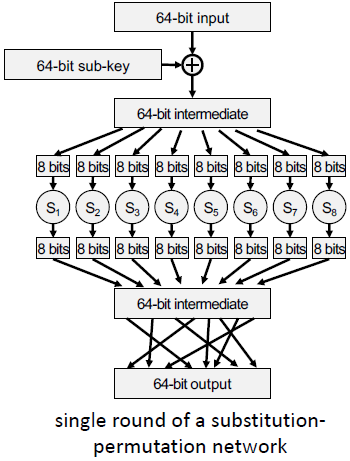
\includegraphics[width=0.4\textwidth]{1.png}
\end{figure}
For this network, we need to do key scheduling, where round key is derived from master key.
\end{definition}
Enough rounds will guarantee an avalanche effect, where small change in the input must affect every bit of the output.\\
However, this substitution permutation network is usually not invertible. However, we have the feistel network to make use of them to construct a invertible function.
\begin{definition}[Fiestel Network]
\hfill\\\normalfont In Fiestel network, we require $f_i$ to be keyed round found from $\{0,1\}^{\frac{l}{2}}\to\{0,1\}^{\frac{l}{2}}$. Then, in teh $i$th round, we have
$
L_i=R_{i-1}\text{ and }R_i=L_{i-1}\oplus f_i(R_{i-1})
$
and inverting $i$th round is
$
R_{i-1}=L_i\text{ and }L_{i-1}=R_i\oplus f_i(R_{i-1})
$
\begin{figure}[h]
\centering
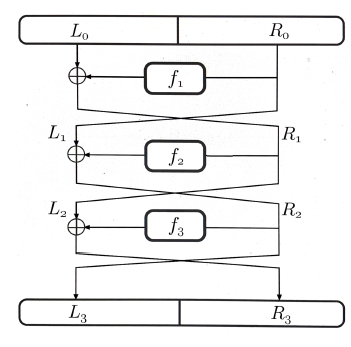
\includegraphics[width=0.4\textwidth]{2.png}
\end{figure}
\end{definition}
\begin{definition}[Data Encryption Scheme]
\hfill\\\normalfont In Data Encryption Scheme, 16 rounds of Feistel netowrk with key length 56 and block length 64 are used. The single round function is illustrated in the figure below.
\begin{figure}[h]
\centering
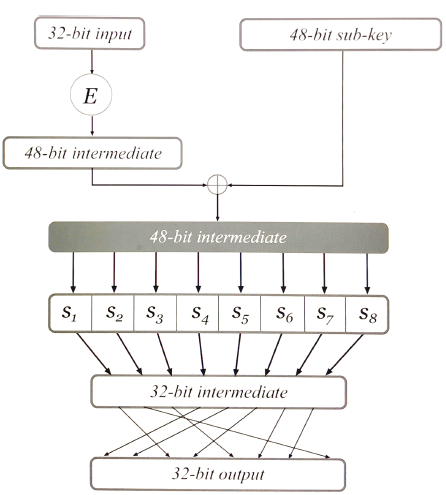
\includegraphics[width=0.4\textwidth]{3.png}
\end{figure}
Here, $E$ is a expansion function, and $S_i$ are $S$ boxes from $6$ bits to $4$ bits, that is non-invertible, publicly known and carefully designed. 
\end{definition}
Since the key length of DES is 56, it is not secure now. Double DES is also not secure due to meet-in-the-middle attack. Triple DES is equivalent to a DES of key length 112 and is still not secure.

\section{Private Key(Symmetric) Cyrptography}
Apart from confidentiality, we also concern about \textbf{integrity} and \textbf{availability}. Under integrity, we have \textbf{user authentication}, which concerns the authenticity of sender, and also \textbf{message authentication}, which concerns the integrity of message.\\Do note that encryption does not ensure integrity:
\begin{itemize}
  \item CTR-mode encryption: ciphertext bit flip will lead to plaintext bit flip
  \item CBC-mode encryption: IV bit flip will lead to first message block bit flip
  \item Perfect secure OTP: Ciphertext bit flip leads to plaintext bit flip
\end{itemize}
\subsection{Message Authentication Code}
Message authentication code is used to prevent adversary from modifying a message sent by one party to another, or from injecting a new message. It requires the sharing of key between communicating parties.\\
Formally, MAC consists of three functions involved with sender and receiver 
\begin{itemize}
  \item \texttt{Gen}: key-generation algorithm
  \item \texttt{Mac}: tag-generation algorithm, which
  \begin{itemize}
    \item Input: a key $k$ and message $m\in\{0,1\}^\ast$.
    \item Output: a tag $t=\texttt{Mac}_k(m)$
  \end{itemize}
  \item \texttt{Vrfy}: verification algorithm, which
  \begin{itemize}
    \item Input: a key $k$, and a message $m$, a tag $t$
    \item Output: bit $b=\texttt{Vrfy}_k(m,t)$, where $b=1$ indicates valid and $0$ indicates invalid
  \end{itemize}
\end{itemize}
For \textit{canonical} verification where \texttt{Mac} is deterministic, receiver's \texttt{Vrfy} function will just recompute $\texttt{Mac}_k(m)$ and compare with tag $t$ received.
\begin{definition}[Existential Unforgeability]
\hfill\\\normalfont Consider the following \textbf{message authentication experiment} $\MacForge_{\mathcal{A}, \Pi}(n)$.
\begin{itemize}
  \item Key $k$ is generated by $\texttt{Gen}(1^n)$.
  \item $\mathcal{A}$ has oracle access to $\texttt{Mac}_k()$ with $Q$, the set of all asked queries. $A$ outputs $(m,t)$.
  \item $\mathcal{A}$ succeeds if and only if 
  \begin{itemize}
    \item $\texttt{Vrfy}_k(m,t)=1$
    \item $m\not\in Q$
  \end{itemize}
\end{itemize}
When $\mathcal{A}$ succeeds, we say $\MacForge_{\mathcal{A},\Pi}(n)=1$.\\
We say a MAC is \textbf{existentially unforgeable} under an adaptive chosen-message attack, if for all PPT adversary $\mathcal{A}$, there is a negligible function \textbf{negl} such that
$
P(\MacForge_{\mathcal{A},\Pi}(n)=1)\leq \mathbf{negl}(n)
$
\end{definition}
It is not a ``too strong'' definition since we want MAC scheme to be application-independent.\\
\textbf{Remark}: MAC is in general \textit{not} designed to detect \textbf{replays}. Replay attack can be prevented via application-dependent schemes such as \textbf{sequence number}, or \textbf{timestamp}.
\begin{definition}[Strong MAC]
\hfill\\\normalfont MAC definition does not allow adversary to forge a different valid tag $t_1'\neq t_1$ on the previously submitted messages. However, adversary may be able to find a valid pair $(m_1,t_1')$. \\
In strong mac, we consider the following message authentication experiment $\MacSForge_{\mathcal{A}, \Pi}(n)$:
\begin{itemize}
  \item Key $k$ is generated by $\texttt{Gen}(1^n)$
  \item $\mathcal{A}$ has oracle access to $\texttt{Mac}_k()$ with $Q$, the set of all asked queries \underline{pairs}. $\mathcal{A}$ outputs $(m,t)$.
  \item $\mathcal{A}$ succeeds if and only if 
  \begin{itemize}
    \item $\texttt{Vrfy}_k(m,t)=1$
    \item $(m,t)\not\in Q$
  \end{itemize}
\end{itemize}
When $\mathcal{A}$ succeeds, we say $\MacSForge_{\mathcal{A},\Pi}=1$.\\
A MAC is a \textbf{strong MAC} under an adaptive chosen-message attack, if for all PPT adversary $\mathcal{A}$, there is a negligible function $\mathbf{negl}$ such that
$
P(\MacSForge_{\mathcal{A},\Pi}(n)=1)\leq \mathbf{negl}(n)
$
A secure MAC using canonical verification is also strongly secure.
\end{definition}
\textbf{Remark}: Authentication enables the receiver to verify origin, but the receiver cannot convince a third party of origin. On the other hand, signature enables the receiver to verify origin and receiver can convince third party of origin as well. The unique property of signature is called \textbf{non-repudiation}.
\subsection{CBC-MAC}
CBC-MAC is the standardized MAC, and is widely used.
\begin{figure}[h]
\centering
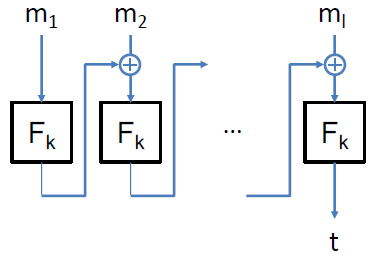
\includegraphics[width=0.4\textwidth]{4.png}
\end{figure}
Here, we define $t_i=F_k(t_{i-1}\oplus m_i)$ and $t_0=0^n$. Output $t_l$ as the tag $t$.\\\texttt{Vrfy} will output 1 if and only if $t=\texttt{Mac}_k(m)$.\\
CBC-MAC is only secure for fixed length messages as \textbf{concatenation attack} is possible for arbitrary length CBC-MAC:
\begin{itemize}
  \item Suppose $(m,t)$ and $(m',t')$ are available
  \item we construct $m''$ to be $m$ followed by $t\oplus m_1'$ followed by rest of $m'$.
  \item Then the output tag will be $t'$ for $m''$.
\end{itemize}
\begin{definition}[Authenticated Encryption]
\hfill\\\normalfont A private-key-encryption scheme is an authenticated encryption scheme if it is (1)CCA-secure and (2)unforgeable.
\end{definition}
Suppose we have 
\begin{itemize}
  \item $\Pi_E=(\texttt{Enc},\texttt{Dec})$, a CPA-secure encryption
  \item $\Pi_M=(\texttt{Mac}, \texttt{Vrfy})$, message authentication code
\end{itemize}
We may have the following three procedures:
\begin{enumerate}
  \item Encrypt-and-authenticate: $c\leftarrow \texttt{Enc}_{k_E}(m)$, $t\leftarrow \texttt{Mac}_{k_M}(m)$\\
  $t$ is deterministic when \texttt{Mac}  is deterministic and therefore it is not CPA-secure
  \item Authenticate-then-encrypt: $t\leftarrow \texttt{Mac}_{k_M}(m)$, $c\leftarrow \texttt{Enc}_{k_E}(m\|\|t)$\\
  This is not necessarily secure. Consider the CBC-mode-with-padding, there are two error cases, which are ``bad pidding'' and ``MAC failure''. The first message may give rise to padding oracle attack.
  \item Encrypt-then-authenticate: $c\leftarrow \texttt{Enc}_{k_E}(m)$, $t\leftarrow \texttt{Mac}_{k_M}(c)$\\
  If $\Pi_E$ is CPA secure and $\Pi_M$ is strong MAC, this scheme then is secure authenticated encryption scheme
\end{enumerate}
The important principle here is that each cryptographic primitives should always use independent keys.
\subsection{Cryptographic Hash Function}
\begin{definition}[Hash Function]
\hfill\\\normalfont Hash Function is function that takes input of arbitrary length and compress them into short, fixed-length outputs. Here, evaluation of $H:\{0,1\}^\ast\to\{0,1\}^l$ should be efficient and public.
\end{definition}
\begin{definition}[Cryptographic Hash Function]
\hfill\\\normalfont Cryptographic Hash Function shuold be a hash function that has
\begin{itemize}
  \item Collision Resistance
  \item Second Preimage Resistance
  \item Preimage Resistance
\end{itemize}
\end{definition}
\begin{definition}[Collision Resistance]
\hfill\\\normalfont Consider $\Pi=(\texttt{Gen}, H)$ where $\texttt{Gen}$ is a key generation algorithm and $H$ a keyed hash function: $H:(s, x)\to \{0,1\}^l$.\\
Define the collision-finding experiment $\text{Hash-coll}_{\mathcal{A},\Pi}(n)$:
\begin{itemize}
  \item key $s$ is generated by \texttt{Gen}
  \item Adversary $\mathcal{A}$ is given key $s$, and will output $x$, $x'$.
  \item $\text{Hash-coll}_{\mathcal{A},\Pi}(n)=1$ if and only if $x\neq x'$ and $H^s(x)=H^s(x')$.
\end{itemize}
$\Pi$ is collision resistant if for all PPT adversary $\mathcal{A}$, there is a \textbf{negl} such that 
$
P(\text{Hash-coll}_{\mathcal{A},\Pi}(n)=1)\leq \textbf{negl}(n)
$
\end{definition}
\textbf{Remark}: Cryptographic hash functions in practice are usually \textbf{unkeyed}.
\begin{theorem}[Hash-And-Mac]
\hfill\\\normalfont Hash-and-Mac uses hash to reduce arbitrary-length message $m$ to a fixed-length digest $H(m)$ and apply a fixed-length MAC, e.g. CBC-MAC.\\
If MAC is secure and hash is collision resistant, the hash-and-MAC is a secure MAC.
\end{theorem}
\begin{definition}[HMAC]
\hfill\\\normalfont Standardized HMAC is formalized as below:
\begin{itemize}
\item \texttt{Gen}: two keys $s$ and $k$
\item \texttt{Mac}: $t=H^s((k\oplus opad) \| H^s((k\oplus ipad)\| m))$
\item \texttt{Vrfy}: Output $1$ if and only if $t$ equals $\texttt{Mac}_{s,k}(m)$ in a canonical sense.
\end{itemize}
\end{definition}
HMAC is highly efficient and supported by proof of security. 
\subsection{Attack on Cryptographic Hash Functions}
Suppose $H:\{0,1\}^\ast \to \{0,1\}^l$ is a collision resistant hash function. Then it takes at least $q:=2^l+1$ hashes to found a collision with probability $1$. However, if we want a collision with probability with probability $0.5$, it takes roughly $2^{\frac{l}{2}}$ hashes to find a pair of duplicates among them with probability $\frac{1}{2}$.
\subsection{Hash Function in Practice}
\begin{itemize}
  \item MD5: 128-bit output. Insecure. Collision found in 2004.
  \item SHA-1: 160-bit output length. Very common. Collision found in 2017.
  \item SHA-2: 256/512 bit output length. No known significant weaknesses
  \item SHA-3: 224,256, 384, 512-bit outputs.
\end{itemize}
Hash Function can be applied in 
\begin{itemize}
  \item Fingerprinting: instead of storing original data, one can stores a short hash digest, such as virus fingerprinting.
  \item Authenticating a sequence of data values: $D_0,\ldots, D_N$. This is done via \textbf{merkle hash trees}.\\
  \begin{figure}[h]
  \centering
  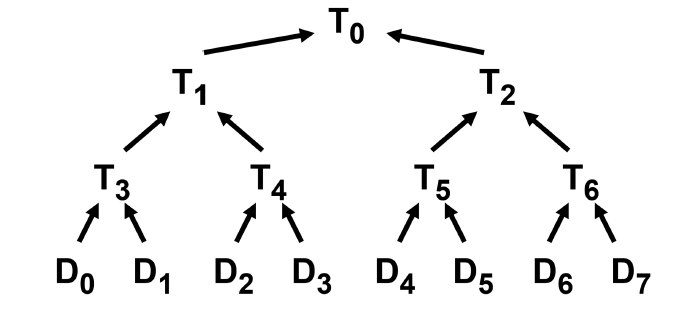
\includegraphics[width=0.4\textwidth]{5.png}
  \end{figure}
  Merkle has tree makes the data the leaves of the tree and take hash recursively until root. Verifier knows $T_0$, the hash at the root. Verifier can authenticate leaf $D_i$, if the person can supply $D_i$ with the elements $D_j$ and $T_k$'s required in obtaining $T_0$ upstream to the root.
  \item Another way to do so in one-way hash chains. 
  \begin{figure}[h]
  \centering
  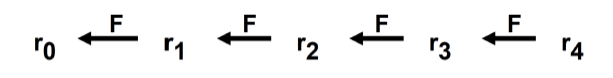
\includegraphics[width=0.4\textwidth]{6.png}
  \end{figure}
  It picks a random $r_N$ with a public \textbf{one-way} function $F$. $r_i$ is calculated by $r_i=F(r_{i+1})$ and $r_0$ will be made public.\\
  It is used in reverse order of construction. Authentication of $r_i$ can be efficiently done given $r_j$ with $j>i$.
  \item Password hashing. Password is stored in terms of hash, since preimage resistance of $H$ makes inverting the hash difficult.\\
  However, password space is quite limited, and there is possibility for pre-computation. Therefore, we should use 
  \begin{itemize}
    \item Slow hash functions, like bcrypt.
    \item Hash password together with a random salt $s$, i.e. $h=H(\text{passwaord}\| s)$ and store $(h,s)$. The salt increases the difficulty for precomputation.
  \end{itemize}
  \item Key Derivation. Suppose there is a shared secret with enough entropy but non-uniform distribution. One can use hash function to obtain a uniform distributed secret key.
  \item Commitment Schemes. Suppose $C(m)$ is the commitment to a value $m$. We can define $C(m)L=h(r\| m)$ to hide content of $m$ from the public, but also binds the bidder with the value $m$. Here, $r$ is a length-$l$ random sequence.\\
  This hash function $h$ requires \textbf{preimage resistence}, \textbf{collision resistance} and \textbf{non-malleability properties}.
\end{itemize}

\section{Cryptographic Hardness Assumptions}
Many private-key cryptography are based on assumption that pseudorandom permutation(PRP) exists. The \textit{existence} of PRP can be proved based on assumption that one-way function exist, whereas the existence of one-way function can be proved if factoring problem is hard.
\subsection{Mathematics Preliminaries}
\begin{theorem}[Greatest Common Divisor]
\hfill\\\normalfont There exists a unique $d\in\mathbb{Z}$ such that for any given $a,b\in\mathbb{Z}$, we have
\begin{itemize}
\item $d\geq 0$
\item $d\mid a$ and $d\mid b$
\item for any $c\in \mathbb{Z}$ such that $c\mid a$ and $c\mid b$, it is true that $c\mid d$.
\end{itemize}
This $d$ is called \textbf{greatest common divisor} of $a$ and $b$.
\end{theorem}
\begin{definition}[Relatively Prime]
if $a,b\in\mathbb{Z}$ and $\gcd(a,b)=1$, then $a,b$ are relatively prime.
\end{definition}
\begin{theorem}\normalfont If $a\mid (bc)$ and $d=\gcd(a,b)=1$, then $a\mid c$.\end{theorem}
\begin{definition}[Modulo]
\hfill\\\normalfont $a\mod N$ is the remainder of $a$ divided by $N$. We have $0\leq a\mod N\leq N-1$.
\end{definition}
\begin{theorem} $a=b\pmod N \Leftrightarrow a\mod N = b\mod N$.\end{theorem}
It is known that integer addition, subtraction, multiplication, division are efficient. It is known that modular addition/subtraction/multiplication/division is efficient. It is known that \textbf{modular exponentiation} is efficient.
\begin{theorem}[Euclid's Algorithm]
\hfill\\\normalfont $\gcd(a,b)=\gcd(b,r)$ if we have $a=q\cdot b+r$ with $0\leq r<b$.\\
Using this, we can find $\gcd(a,b)$ in polynomial time.
\end{theorem}
\begin{definition}[Abelian Group]
\hfill\\\normalfont An abelian group is a set $G$ and a binary operation $\circ$ defined on $G$ such that
\begin{itemize}
  \item $\forall a, b\in G, a\circ b \in G$.
  \item $\exists e\in G$ such that $\forall g\in G, e\circ g=g$. $e$ is called identity.
  \item Every $g\in G$ has inverse $h\in G$ such that $h\circ g = e$. Here the inverse is called left inverse.
  \item For all $f,g,h\in G$, $f\circ(g\circ h)=(f\circ g)\circ h$. This is associativity.
  \item For all $g,h\in G$, $g\circ h=h\circ g$. This is commutativity.
\end{itemize}
We define the \textbf{order} of a finite group $G$ by the number of elements in $G$.
\end{definition}

An additive abelian group supports the operation $+$ with an identity denoted by $0$. Inverse of $g$ is denoted by $-g$ and group exponentiation is denoted by $m\cdot a$.\\
An multiplicative abelian group supports the operation $\times$ with an identity denoted by $1$. Inverse of $g$ is denoted by $g^{-1}$ and group exponentiation dentoed by $a^m$.

\begin{theorem}[{$\mathbb{Z}_{N}$}]
\hfill\\\normalfont $\mathbb{Z}_{N}$ is a additive group under addition modulo $N$.
\end{theorem}
\begin{definition}{Modular Inverse}
\hfill\\\normalfont $b$ is invertible modulo $N$ if there eixsts an element $b^{-1}$ such that $b\cdot b^{-1}=1\mod N$. It is known that $b^{-1}$ is unique mod $N$ if it exists.
\end{definition}
\begin{theorem}[Existence Condition of Modular Inverse]
\hfill\\\normalfont $b$ is invertible modulo $N$ if and only if $\gcd(b,N)=1$.
\end{theorem}
\begin{theorem}[{$\mathbb{Z}^\ast_{N}$}]
\hfill\\\normalfont $\mathbb{Z}_N^\ast$ is a group with invertible elements between $1$ and $N-1$ under multiplication modulo $N$.
\end{theorem}
\begin{definition}[Euler's Totient Function]
\hfill\\\normalfont $\varphi(N)$ is the Euler's totient function, which measures the number of invertible elements modulo $N$.\\
$\varphi(N)=N-1$ if $N$ prime. If $N=pq$ where $p,q$ are primes, then $\varphi(N)=(p-1)(q-1)$.
\end{definition} 
\begin{theorem}[Fermat's Little theorem]
\hfill\\\normalfont Let $G$ be finite group of order $m$. Then for any $g\in G$, we have
$
g^m=1
$
\end{theorem}
Specifically, for all $z\in\mathbb{Z}_N$, we have $N\cdot a=0\mid N$ and for all $z\in \mathbb{Z}_N^\ast$, we have $a^{\varphi(N)}=1\mod N$.
\begin{theorem}\normalfont Let $G$ be finite gorup of order $m$. Then for $g\in G$ and $x\in \mathbb{Z}$, it holds that $g^x=g^{x\mod m}$.
\end{theorem}
\begin{theorem}\normalfont Let $G$ be finite group of order $m$. We define $f_e$ to be $f_e(g)=g^e$ for any integer $e$, where $g\in G$. If $\gcd(e,m)=1$, then $f_e$ is permutation. Also if $d=e^{-1}\mod m$, then $f_d$ is inverse of $f_e$.
\end{theorem}
\subsection{Factoring and RSA Problem}
It is common sense that multiplying two numbers is easy, but factoring a number is hard. Among all numbers, the hardest numbers to factor are those that are the products of two equal-length primes.\\
The factoring problem is related to RSA problem. RSA problem involves $\mathbb{Z}_N^\ast$. where $N=p\times q$, $p,q$ primes. The order of $\mathbb{Z}_N^\ast$ is $\varphi(N)=(p-1)(q-1)$. This order is easy to compute if $p,q$ known and hard to compute otherwise. Therefore, computing $\varphi(N)$ is as hard as factoring $N$.\\
Fix $e$ with $\gcd(e,\varphi(N))=1$, then we known exponentiation to the $e$th power is a permutation of $\mathbb{Z}_N^\ast$, and there exists a unique $d$, which satisfies $ed=1\mod \varphi(N)$, that gives $(x^d)^e=x\mod N$. We call $x^d$ $e$th root of $x$ modulo $N$.\\
As long as $p,q$ is known or $\varphi(N)$ is known which implies $p,q$ can be computed in polynomial time, then we can compute $x^d$ easily. Otherwise, computing $d$ is as hard as factoring $N$.
\begin{definition}[RSA Problem Relative to GenRSA]
\hfill\\\normalfont We first define a experiment called GenRSA.\\
GenRSA: On input $1^n$, outputs $(N,e,d)$ with $N=pq$, a product of two $n$-bit primes, and with $ed=1\mod \varphi(N)$. Then, the experiment $\text{RSA-inv}_{\mathcal{A}, \text{GenRSA}}(n)$ is defined as below:
\begin{itemize}
  \item Compute $(N,e,d)\leftarrow \text{GenRSA}(1^n)$
  \item Choose uniform $y\in \mathbb{Z}_N^\ast$.
  \item Run $\mathcal{A}(N,e,y)$ to get $x$.
  \item Experiment evaluates to $1$ if $x^e=y \mod N$.
\end{itemize}
The RSA problem is relative to GenRSA if for all PPT algorithm $\mathcal{A}$, we have $P(\text{RSA-inv}_{\mathcal{A}, \text{GenRSA}}(n)=1)<\mathbf{negl}(n)$.
\end{definition}
In layman's words, given $N$ and $e$, it is hard to compute the $e$th root of a uniform element $y\in\mathbb{Z}_N^\ast$.\\
\begin{definition}[Rough Sketch of Implementation of GenRSA]
\hfill\\\normalfont To implement GenRSA,
\begin{itemize}
  \item Generate uniform $n$-bit primes $p,q$.
  \item Set $N=pq$.
  \item Choose arbitrary $e$ with $\gcd(e,\phi(N))=1$.
  \item Compute $d=e^{-1}\mod \varphi(N)$.
  \item Output $(N,e,d)$.
\end{itemize}
It is worth noting that choice of $e$ does not affect hardness of RSA problem, therefore common choices can be $e=3$ or $e=2^{16}+1=65537$.
\end{definition}
\begin{theorem}[Hardness of RSA relative to Factoring]
\hfill\\\normalfont If factoring moduli output by GenRSA is easy, then RSA problem must be easy relative to GenRSA.\\
However, the RSA problem is not known to be implied by hardness of factoring.
\end{theorem}
\subsection{Cyclic Group, Discrete Logarithm Problem}
\begin{definition}[Cyclic Group]
\hfill\\\normalfont Let $G$ be a finite group of order $m$. Let $g$ be an element of $G$. Consider the set $S=\{g^0, g^1,\ldots\}$. If the set $S$ has $m$ elements, then $G=S$, and we say such $G$ is a cyclic group and such $g$ is a generator of $G$.
\end{definition}
\begin{theorem}[Prime Order Group is Cyclic]
\hfill\\\normalfont Any group of prime order is cyclic, and every non-identity element is a generator.
\end{theorem}
\begin{theorem}\normalfont If $p$ is a prime, the $\mathbb{Z}_p^\ast$ is cyclic.\end{theorem}
It is also worth noting, it is easy to do uniform sampling in cyclic group $G$. Given $G$ is of order $m$ and a generator $g$, to sample uniformly an element $h\in G$, choose uniformly $x\in\{0,\ldots, m-1\}$ and set $h=g^x$.
\begin{definition}[Discrete Logarithm Problem]
\hfill\\\normalfont Let $\mathcal{G}$ be a group-generation algorithm. Specifically, on input $1^n$, $\mathcal{G}$ outputs a cyclic group $G$ with order $q$ such that $\|q\|=n$ and a generator $g$.\\
For algorithm $\mathcal{A}$, define experiment $\text{Dlog}_{\mathcal{A}, \mathcal{G}}(n)$:
\begin{itemize}
  \item Compute $(G,q,g)\leftarrow \mathcal{G}(1^n)$.
  \item Choose uniform $h\in G$.
  \item Run $\mathcal{A}(G,q,g,h)$ to get $x$.
  \item And experiment evalutaes to $1$ if $g^x=h$.
\end{itemize}
The discrete-logarithm problem is hard relative to $\mathcal{G}$ if for all PPT algorithm $\mathcal{A}$, $P(\text{Dlog}_{\mathcal{A},\mathcal{G}}(n)=1)<\mathbf{negl}(n)$.
\end{definition}
\subsection{Diffie-Hellman Problem}
\begin{definition}[Diffie-Hellman Problem]
\hfill\\\normalfont Here we fix cyclic group $G$ with generator $g$. Suppose $h_1 = g^x,h_2=g^y\in G$, then define $\text{DH}_g(h_1,h_2)=DH(g^x,g^y)=g^{xy}$.\\
For \textit{computational} Diffie-Hellman problem, given $g,h_1,h_2$, compute $\text{DH}_g(h_1,h_2)$.\\
For \textit{decisional} Diffie-Hellman problem, given $g,h_1,h_2$, distinguish the correct $\text{DH}_g(h_1, h_2)$ from a uniform element of $G$. And the DDH problem is hard relative to $\mathcal{G}$ if for all PPT algorithm $\mathcal{A}$, we have
$
|P[A(G,q,g,g^x,g^y,g^z)=1]-P[A(G,q,g^x,g^y,g^{xy})=1]|\leq \mathbf{negl}(n)
$
\end{definition}
\begin{theorem}[Relative Difficulty of Diffie-Hellman Problems]
\hfill\\\normalfont It is known that, relative to $G$:
\begin{itemize}
  \item If DL is easy, so is CDH;
  \item If CDH is easy, so is DDH.
\end{itemize}
\end{theorem}

\section{Public Key Cryptography}
The notion of public-key cryptography involves a pair of keys $(pk, sk)$, where
\begin{itemize}
  \item $pk$, the public key is widely disseminated
  \item $sk$, the private key is kept secretly
\end{itemize}
Here, $pk$ is used for encryption and $sk$ is for decryption in encryption scheme; $sk$ is used for signature and $pk$ is for verification in authentication scheme.\\
Here, we need to assume that $pk$ is disseminated via an authenticated channel. This assumption will be removed in the future.\\
One consequence is that anyone with $pk$ is able to encrypt message but only the one with $sk$ can decrypt message.\\
Another thing is that signature using $sk$ will provide non-repudiation property.
\subsection{RSA Encryption}
\begin{definition} [Public Key Encryption]
\hfill\\\normalfont Public key encryption scheme is a triple $(\texttt{Gen}, \texttt{Enc}, \texttt{Dec})$, where
\begin{itemize}
  \item \texttt{Gen}: key-generation algorithm that outputs $(pk, sk)$;
  \item \texttt{Enc}: encryption algorithm $c:=\texttt{Enc}_{pk}(m)$
  \item \texttt{Dec}: decryption algorithm $m:=\texttt{Dec}_{sk}(c)$.
\end{itemize}
\end{definition}
Since, encryption uses $pk$ which the public has, \textbf{CPA} security is the baseline security notion.\\
Deterministic public-key encryption, such as student RSA, cannot be CPA secure. This is because
\begin{itemize}
  \item One can determine repeated encryption of a plaintext
  \item It may allow adversaries to recover plaintext messages when message set is small.
\end{itemize}
For CCA definition, adversay is allowed to have access to decryption oracle as well.
\begin{definition}[Textbook RSA]
\hfill\\\normalfont For textbook RSA, we define the triplet as 
\begin{itemize}
  \item \texttt{Gen}: $(N,e,d)\leftarrow \text{GenRSA}(1^n)$. Here, $(N,e)$ is the public key, and $(N,d)$ is private key.
  \item \texttt{Enc}: for $m\in \mathbb{Z}_N^\ast$, compute $c:=m^e\mod N$.
  \item \texttt{Dec}: given $c\in\mathbb{Z}_N^\ast$, compute $m:=c^d\mod N$.
\end{itemize}
\end{definition}
This textbook RSA is insecure, as we can use common-modulus attack.
\begin{itemize}
  \item Common modulus attack 1
  \item Common modulus attack 2\\
  Several users share $N$, and suppose $\gcd{e_1,e_2}=1$. Afversary can see $c_1=m^{e_1}\mod N$ and $c_1=m^{e^2}\mod N$ of the same message $m$. Since $\gcd(e_1,e_2)=1$, there exists $x,y$ such that $xe_1+ye_2=1$. Therefore, adversary computes $c_1^xc_2^y=m\mod N$ and gets the plaintext.
\end{itemize}
In CCA notion, we can also have CCA attack.
\begin{itemize}
  \item CCA attack 1\\
  Adversary obtains a user's ciphertext $c=m^e\mod N$, picks a random $r\in\mathbb{Z}_N^\ast$ and creates forgery $c'=r^ec\mod N$. It submits $c'$ for decryption, and gets back $m'$. Then $m=m'r^{-1}\mod N$.
  \item CCA attack 2\\
  Adversary obtains a user's ciphertext $c=m^e\mod N$ of a unknown $m$. It is easy to generate $c'$ that is an encryption of $2m\mod N$, by just setting $c'=2^ec\mod N$.
\end{itemize}
\begin{definition}[Optimal Asymmetric Encryption Padding(OAEP)]
\hfill\\\normalfont This optimal asymmetric encryption padding provides RSA-based CCA-secure encryption.
\begin{figure}[h]
\centering
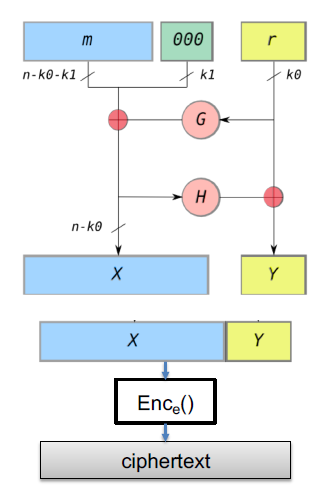
\includegraphics[width=0.2\textwidth]{7.png}
\end{figure}
Here, $G,H$ are independent hash functions, $r$ a unique random number per encryption.
\end{definition}
\begin{theorem}[Checking Primality]
\hfill\\\normalfont We have $a^{p-1}=1\mod p$ where $0<a<p$ if $p$ is a prime. The other direction is not true.\\
However, if $a^{p-1}=1\mod p$ holds, and $p$ is long, then propability that $p$ is not a prime is small(100 digit $p$, $10^{-13}$ probability). Therefore, to further ensure correctness, try multiple values of $a$.\\
\textbf{Caveat}: Carmichael numbers. There exists $p$ such that $p$ not prime and $a^{p-1}=1\mod p$ for all choices of $0<a<p$.\\
Another useful theorem: if $p$ is odd prime, then $x^2=1\mod p$ has only two solutions, namely $x=1$ and $x=-1$. So we can use its contrapositive to see whether a number $p$ is not prime.
\end{theorem}

\section{Diffie Hellman and El Gamal}
Recall the special cyclic group $\mathbb{Z}_p^\ast$ where $p$ is a prime. \textit{Not every} element of $\mathbb{Z}_p^\ast$ is a generator. 
\begin{definition}[Order of Element in {$\mathbb{Z}^\ast_p$}]
\hfill\\\normalfont For any $x\in \mathbb{Z}^\ast_p$, the order of $x$ is the \textbf{smallest} positive integer $a$ such that $x^a=1\mod p$.
\end{definition}
\begin{theorem}\normalfont For all $x\in\mathbb{Z}^\ast_p$, the order of $x$ divides $p-1$.
\end{theorem}
\begin{definition}[Quadratic Residue]
\hfill\\\normalfont An element $x\in \mathbb{Z}^\ast_p$ is called a \textbf{quadratic residue}(QR) if its square root exists in $\mathbb{Z}^\ast_p$.
\end{definition}
\begin{theorem}\normalfont Each element $x\in \mathbb{Z}^\ast_p$ has either $0$ or $2$ square roots.\\
Specially, if $x=a^2\mod p$, then so is $x=(-a)^2\mod p$.
\end{theorem}
\begin{theorem}\normalfont Exactly half of the elements in $\mathbb{Z}^\ast_p$ are quadratic residue.\\
This is due to the square root-able of $g^{k}$, where $g$ generator if and only if $k$ is even.
\end{theorem}
It is konwn that, if given $x\in \mathbb{Z}^\ast_p$, deciding whether $x$ is a quadratic residue is computationally \textbf{easy}. It can be checked using Legendre symbol.
\begin{theorem}[Legendre Symbol]
\hfill\\\normalfont Define Legendre symbol $\mathcal{L}_p(x)=x^{\frac{1}{2}(p-1)}\mod p$. It is known that
$
\mathcal{L}_p(x)=\begin{cases}
1 & \text{ if }x\text{ is a QR}\\
-1& \text{ if }x\text{ is not a QR}\\
0 \text{ if }x=0\mod p
\end{cases}
$
An useful property is
$
\mathcal{L}_p(xy)=\mathcal{L}_p(x)\mathcal{L}_p(y)
$
\end{theorem}
Also, computing square roots in $\mathbb{Z}^\ast_p$ is also computationally feasible. It is known that $O(n^4)$ randomized algorithm exists.\\
However,
\begin{theorem}\normalfont Discrete Logarithm(DL) is in general a computationally \textbf{hard} problem in cyclic groups.
\end{theorem}
\subsection{Discrete Logarithm(DL) problem}
Recall the Discrete Logarithm problem: let $g$ be a generator of cyclic group. Given $x\in G$ find exponent $e$ such that $x=g^e$.\\
The DL problem has a similar form of RSA problem:\\
\textbf{RSA}: given $n$, $e$, $y$, find $x$ such that $x^e=y\mod n$.\\
\textbf{DL}: given $n$, $x$, $y$, find $e$ such that $x^e=y\mod n$.\\
\subsection{Diffie-Hellman Key Exchange}
The aim is to establish a \textbf{common secret} key over an \textbf{unsecured} channel with presence of \textbf{eavesdropper}.\\
\begin{definition}[Diffie Hellman Key Exchange]
\hfill\\\normalfont Suppose Alice and Bob pre-determine a set of \textbf{public parameters}: a prime $p$ and a generator $g$ of $\mathbb{Z}_p^\ast$.
\begin{enumerate}
  \item Alice chooses a random $x$ and computes $c:=g^x\mod p$.\\Alice sends $c$ to Bob.
  \item Bob chooses a random $y$ and computes $d=g^y\mod p$. Bob sends $d$ to Alice.
  \item Bob computes the secret key $k=c^y\mod p$.
  \item Alice computes the secret key $k=d^x\mod p$.
\end{enumerate}
Essentially, the established key $k=g^{xy}\mod p$.
\end{definition}
It is obvious that we need to make it hard to determine $k:=g^{xy}\mod p$ given $g^x$, $g^y$, $p$ and $g$.
\begin{definition}[Computational Diffie-Hellman]
\hfill\\\normalfont \textbf{Computational Diffie-Hellman Problem(CDH)}: Let $g$ be generator of a cyclic group $G$. Given $g^a$, $g^b$, find $g^{ab}$.
\end{definition}
CDH is conjectured to be computationally hard in $\mathbb{Z}_p^\ast$ in general. \\
If CDH is easy, then adversary of DH key exchange can easily recover the key.
\begin{theorem}\normalfont If DL is easy, so is CDH problem.
\end{theorem}
\begin{definition}[Decisional Diffie Hellman Problem(DDH)]
\hfill\\\normalfont Let $g$ be a generator of a cyclic group $G$. Given a $3$-tuple $(x,y,z)$ of elements from $G$, distinguish whether it is generated by process $A$ or $B$, where
\begin{itemize}
  \item $A$: randomly pick $a,b,c$ from $G$, and outputs $(x:=g^a, y:=g^b, z:=g^c)$.
  \item $B$: randomly pick $a,b$ from $G$, and outputs $(x:=g^a, y:=g^b, z:=g^{ab})$.
\end{itemize}
\end{definition}
\begin{theorem}\normalfont If $G$ is to be used for DH key exchange protocol, DDH problem should be hard for this group $G$.
\end{theorem}
This is because we want to make the obtained session key to be indistinguishable from random, as it is usually used for private key encryption.
\begin{theorem}[DDH NOT Hard for {$\mathbb{Z}_p^\ast$}]
\hfill\\\normalfont For the group $\mathbb{Z}_p^\ast$, DDH is not hard.\\
Note, if $\mathcal{L}_p(z)=\mathcal{L}_p(x)\mathcal{L}_p(y)$, both $A$ and $B$ are possible; otherwise, only $A$ is possible. Therefore, the chance of distinguishing $A$ from $B$ is non-negligible.\\
To solve this, we need to pick $a, b$ that are even. Equivalently speaking, we need every element $x,y,z$ for both $A$ and $B$ to be quadratic residue.
\end{theorem}
\begin{theorem}\normalfont DDH is hard for quadratic residues modulo a prime $p$.\end{theorem}
\begin{theorem}[RSA Key Exchange]
\hfill\\\normalfont Key exchange in presence of eavesdropper can also be done using RSA. 
\begin{enumerate}
  \item Alice randomly chooses the public key and a parameter of RSA, i.e., $N$ and $e$, and sends them to Bob but keeps the private key secret.
  \item Bob randomly picks a session key $k$, encrypts it using public key and sends the ciphertext to Alice. That is, Bob sends
  $
c=k^e\mod N
  $
  \item Alice uses her private key $d$ to encrypt the ciphertext $c$ and obtain $k$.
\end{enumerate}
\end{theorem}
There are two major differences of DH and RSA:
\begin{enumerate}
  \item RSA-based key exchange does not achieve forward secrecy. 
  \begin{itemize}
    \item RSA-based key exchange, if private key $d$ for Alice is compromised in future, all previous session keys can be recovered.
    \item However, in DH-based key exchange, compromise of Alice's private key $x$ in the future does not reveal previous session keys since Bob's key $y$ also contribute to session key generation.
  \end{itemize}
  \item In RSA-based key exchange, Bob selects a session key.
  \begin{itemize}
    \item If it is weak, e.g., not pseudorandom, it can be problematic.
    \item In DH-based key exchange, both Alice and Bob contribute to the key generation and thus such vulnerability has less impact.
  \end{itemize}
\end{enumerate}
\subsection{Man-In-The-Middle(MITM) Attack Against DH Key Exchange}
Imagine Mallory $M$ is a malicious attacker in between Alice and Bob that can modify messages. $M$ can carry out the MITM attack by sending his public key $g^z$ to both parties, so that 2 different session keys are established between Mallory and Alice and Bob respectively.
\begin{figure}[h]
\centering
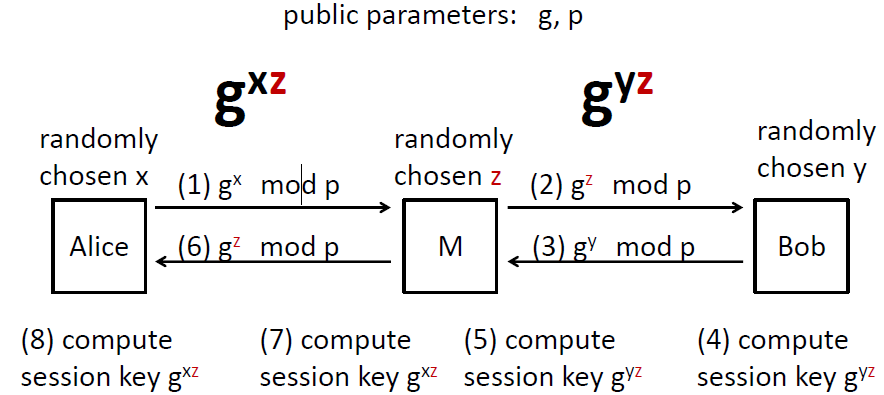
\includegraphics[width=0.4\textwidth]{8.png}
\end{figure}
\subsection{ElGamal Cryptosystem}
In ElGamal Cryptosystem, any party will have 
\begin{itemize}
\item a private key $x$, and
\item a public key $g$, which is the generator $g$ of a cyclic group , and $h:=g^x$.
\end{itemize}
Encryption of message $m$:
$
E(m)=\langle mh^r,g^r\rangle
$
where $m$ must be an element in the cyclic group and $r$ is randonly chosen.\\
Decryption:
$
D(\langle a,b\rangle)=ab^{-x}
$
\begin{theorem}[Security of ElGamal]
\hfill\\\normalfont \begin{itemize}
\item If attacker can solve \textbf{DL}, he can calculate $x$ from $g,h$. Then attacker can decrypt any message.
\item If attacker can solve \textbf{CDH}, he can find plaintext, given $g,h$ and ciphertext.\\
This is because one can compute $h^r$ easily, which allows one to compute $m$.
\item If attacker can solve \textbf{DDH}, then cryptosystem is not semantically secure, or equivalently speaking, not CPA secure.\\
First note, DDH is easy in $\mathbb{Z}_p^\ast$. Also, ElGamal encryption is probabilistic.\\
To be semantically secure, the following problem has to be difficult: the adversary knows that plaintext $m$ is either $g$ or $1$, given public key and ciphertext, $h=g^x, \langle b:=mg^{rx}, c:=g^r\rangle$, the adversary wants to determine the plaintext.\\
Adversay can use DDH to check whether $h,b,c$ are consistent. If consistent, message $m=1$. Otherwise $m=g$.
\end{itemize}
Therefore, to achieve semantic security, one should choose a group where DDH is hard, and use that to construct ElGamal cryptosystem.\\
For example, pick $g\in QR_p\subset\mathbb{Z}_p^\ast$. Take group generated by $g$ as the underlying group in ElGamal.
\end{theorem}
Note, ElGamal in $QR_p$ is CPA secure.\\
Elliptic Curve Cryptography(ECC) is basically ElGamal with another choice of cyclic group.

\section{Digital Signature Algorithm}
Signature scheme usually admits the has-and-sign pattern. Where we have $m\to h(m)\to s(h(m))$, the cryptographic hash function $h$ reduces the size of message $m$ to a small, fixed-sized digest. Then we use $s$ and $\texttt{vrfy}$ to sign or verify, which is more costly than hash function $h$.
\begin{definition}[Digital Signature Algorithm]
\hfill\\\normalfont DSA is based on ElGamal's signature scheme. It requies two primes $p,q$, where $p$ is 512,1024,2048 or 3072 bits and $q$ 160, 224, 256 bits.\\
We use SHA-1, SHA-2 to hash the message. \\
Let us take $p$ to be 1024 bit and $q$ 160 bits. The size of signature is 3320 bits as a result.\\
The public key is $p(1024), q(160), g(1024), y(1024)$ and private key $x(160)$.\\
We require
\begin{itemize}
  \item $p,q$ to be two primes such that
  \begin{itemize}
    \item $q\mid p-1$ and $q^2\mid p-1$.
  \end{itemize}
  \item $g$ a generator in $\mathbb{Z}_p^\ast$ having order $q$.
  \item Let $h:\{0,1\}^\ast\to\mathbb{Z}_q$ a collision resistant hash function.
  \item Set private key be a \textit{randomly chosen} $x\in\mathbb{Z}_q^\ast$.
  \item Set $p,q,g$ public, together with $y:=g^x\mod p$.
\end{itemize}
For \texttt{sign}, given a message $m\in\{0,1\}^\ast$,
\begin{itemize}
  \item Choose $k\in\mathbb{Z}_q^\ast$ uniformly at random
  \item Compute $r=(g^k\mod p)\mod q$.
  \item Compute $s=(h(m)+x\cdot r)\cdot k^{-1}\mod q$
  \item the signature for $m$ is $(r,s)$.
\end{itemize}
For \texttt{Vrfy}, given a message $m\in\{0,1\}^\ast$ and a signature $(r,s)$,
\begin{itemize}
  \item Compute $u_1:=h(m)\cdot s^{-1}\mod q$
  \item Compute $u_2:=r\cdot s^{-1}\mod q$
  \item Output \texttt{YES} if and only if $r=((g^{u_1}y^{y_2}\mod p)\mod q)$.
\end{itemize}
\end{definition}
\textbf{Remark}: 
\begin{enumerate}
  \item Signing can be very fast with precomputation, since $k$, $k^{-1}$ and $r$ can be precomputed before seeing $m$.
  \item Extra care must be taken in choosing $k$ in implementing dsa. It must have high entropy, be unpredictable and unique.
\end{enumerate}
\subsection{Public Key Infrastructure(PKI)}
\begin{definition}[Digital Certificate]
\hfill\\\normalfont Digital certificate is a signature that binds an entity to some public key.\\
For eaxmple, $\text{cert}_{C\to A}$ is a certificate for $A$'s public key issued by $C$. In the certificate, we include $\texttt{sign}_{sk_C}(A\text{'s key is }pk_A)$ in the certificate.
\end{definition}
If $B$ knows $C$'s key $pk_C$ and \textbf{trust} $C$. Then $B$ can believe that $pk_A$ is indeed $A$'s key.\\
In real life, $B$ can be treated as the certificate authority, which keeps the pairings of entity and their public key and creates certificate signed by $B$'s private key.\\
There are two PKI models:
\begin{enumerate}
  \item \textbf{Single CA}: everybody in the system trusts the single CA. The public key of the CA $pk_{CA}$ is installed on everyone's machine over authenticated channel.
  \item \textbf{Multiple CA}: Multiple CAs issue certificate, so as to prevent single point of failure. However, the entire PKI is as insecure as the \textit{weakest} CA.
  \item \textbf{Delegated CAs}: CA can delegate its ability to issue certificates, so that CA's are arranged in a hierarchical structure, with the root CA as the root of the hierarchy.
\end{enumerate}
There are several scenarios where we need to invalidate certificates, for example
\begin{itemize}
  \item Expiration, which can be done by adding an expiration date in the CA and signed
  \item Revocation, which can be done by adding a serial number to the CA and use a published \textbf{Certificate Revocation List} to invalidate.
\end{itemize}
\subsection{Transport Layer Security}
Transport Layer Security is used in \texttt{HTTPS} connections. The TLS handshake is outlined in the diagram below.
\begin{figure}[h]
\centering
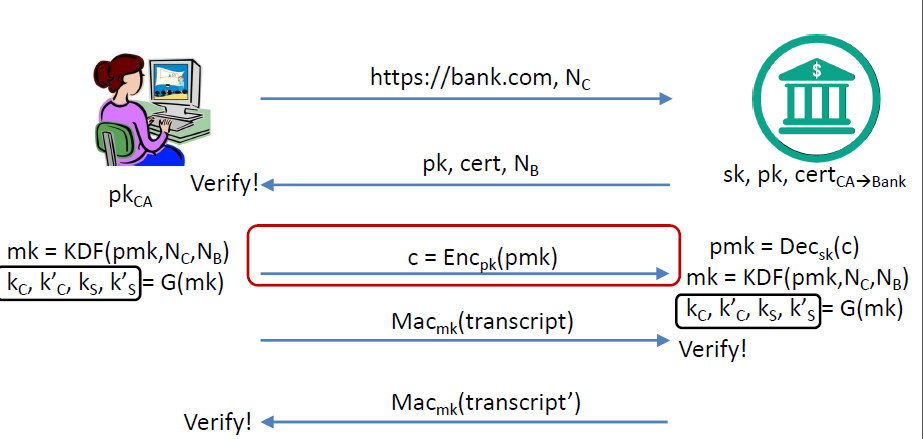
\includegraphics[width=0.4\textwidth]{9.png}
\end{figure}
For the boxed part, the key exchange can be done in different key exchange protocol.
\begin{itemize}
  \item \textbf{RSA}: no forward secrecy
  \item \textbf{Fixed Diffie Hellman}: $S$ has fixed DH key $x_s$; $S$'s DH public key $g^{x_s}$ is included in the certificate. The certificate include bank's public key and DH key. For $C$, it also uses $x_C$ and $g^{x_C}$ so that $C$ and $S$ can execute standard DH protocol.
  \item \textbf{Ephemeral Diffie-Hellman}: Both $S$ and $C$ create fresh secret keys for new sessions. $S$' DH public key $g^{x_S}$ is signed by $S$'s RSA private key. Then $C$ and $S$ carry standard DH protocol to generate a fresh $pmk$.
\end{itemize}
For record-layer protocol, since parties now share $k_C,k_C', k_S, k_S'$, these key can be used for encryption and authentication. It prevents reflection attacks. Sequence numbers can be used to prevent replay attacks.

\section{Digital Cash and Shamir's Secret Sharing}
For today's digital cash, we hope that we can achieve
\begin{itemize}
  \item Only a previously withdrawn coin can be deposited
  \item Coins must be impossible to deposit twice
  \item Shop accept withdrawn coins
  \item Pay is done anonymously
  \item Vendor is assured Bank will accept a payment received from the buyer
\end{itemize}
Currently, we cannot acheive anonymous payment, since it requires 
\begin{itemize}
\item the bank be impossible to trace a coin
\item us to protect honest customer's privacy AND preventing misuse
\end{itemize}
\begin{definition}[Blind Signature]
\hfill\\\normalfont Blind signature requires the signer to sign a message \textit{without} seeing its content. Later when message and signature are revealed, the signer should not be able to link the signature with the corresponding signing transaction. However, the signature needs to be verifiable by everyone.
\end{definition}
We introduce Schnorr's identification protocol, which is the fundamental of Schnorr's blind signature.
\begin{theorem}[Schnorr's Identification Protocol]
\hfill\\\normalfont Let $p,q$ be large primes that satisfies
$
q\mid p-1
$
Let $G_q$ be the subgroup of order $q$ in $\mathbb{Z}_p^\ast$. Let $g$ be a generator of $G_q$. (A special choice of $p,q,G_q$ is actually $G_q=QR_p$, and $p=2q+1$)\\
Let $H:\{0,1\}^\ast\to\mathbb{Z}_p^\ast$ be a collision-resistant hash.\\
We set the \textbf{prover's} secret key $x$ to be $x\in\mathbb{Z}_q$. Its public key is a tuple:
$
(p,q,g,y:=g^x)
$
The Schnorr's identification protocol wants to achieve that the veritifier is convinced that prover has the private key $x$ corresponding to $y$ without learning $x$.:
\begin{itemize}
  \item Prover chooses $r\in \mathbb{Z}_q$, and sends $a:=g^r$ to verifier
  \item Verifier chooses $c\in\mathbb{Z}_q$, and sends it to prover
  \item Prover computes $b=r-cx$ and sends it to verifier.
  \item Verifier accepts the proof if $a=g^by^c$. Otherwise reject.
\end{itemize}
\end{theorem}
\begin{theorem}[Schnorr's Signature]
\hfill\\\normalfont The signer will have the same setting as identification protocol. Upon signing the message $m$, he will produce a pair $(c,b)$ where
$
c:=h(m\| a)
$
and 
$
b=r-cx
$
The signature can be verrified by checking $c=h(m\| g^b y^c)$.
\end{theorem}
This allows the signature scheme to be non-interactive. This scheme relies on the hardness of discrete logarithms of elements of $G_q$.\\
Suppose we have observed a valid transcript $(a',c',b')$ of a Schnorr's identity protocol execution. Consider the transform below:
\begin{itemize}
  \item $u,v,w\in\mathbb{Z}_q$.
  \item $a:=a^{\prime u}g^vy^w$
  \item $c=uc'+w$
  \item $b=ub'+v$
\end{itemize}
The $(a,c,b)$ will be another accepting transcript of Schnorr's identity protocol. With this observation, we can devise Schnorr's blind signature.
\begin{theorem}[Schnorr's Blind Signature]
\hfill\\\normalfont Let the signer's setting to remain the same.
\begin{itemize}
  \item Signer picks a $r'\in\mathbb{Z}_q$ and sends $a':=g^{r'}$ to verifier.
  \item Verifier initialize $u,v,w\in\mathbb{Z}_q$, compute $a:=a^{\prime u}g^v y^w$. It let $c=h(m\| a)$ and $c'=(c-w)u^{-1}$. It sends $c'$ to signer.
  \item Signer returns $b':=r'-c'x$ to verifier.
  \item Verifier computes $a':=g^{b'}y^{c'}$ and $b:=ub'+v$. It verifies whether $(c,b)$ is valid Schnorr's signature.
\end{itemize}
This is good since signer does not learn $m$, $(c,b)$. Also, verifier does not learn $x$. However, anyone can verify $(c,b)$.
\end{theorem}
\begin{theorem}[RSA BBlind Signature]
\hfill\\\normalfont Let Signer's secret key be $(N,d)$ and public key be $(N,e)$.\\
The verifier will pick $r\in\mathbb{Z}_N^\ast$ and compute $m'=H(m)r^e\mod N$. Verifier sends $m'$ to signer.\\
The signer will compute $x':=(m')^d\mod N$ and sends $x'$ to verifier.\\
Verifier will compute $x=r^{-1}x'\mod N$, which is the ordinary RSA signature.
\end{theorem}
\subsection{Splitting Secret Information}
We hope the secret can be split in an information-theoretic way.
\begin{definition}[Threshold Secret Sharing Scheme]
\hfill\\\normalfont Let $t,w$ be positive integers where $t\leq w$. A $(t,w)$-threshold scheme is a method of sharing a secret $K$ among a set of $w$ participants, in such a way that any $t$ participants can compute the value of $K$ but no group of $t-1$ participants can do so.\\
Let $P_1,\ldots, P_w$ be participants, and let the data held by $P_i$ be $s_i$. We assume that there is a dealer who computes the \textit{shares} from $K$ and securely sends the shares to the participants. 
\end{definition}
\begin{theorem}[{$(t,w)$}-Shamir Threshold Scheme]
\hfill\\\normalfont \textbf{Initialization Phase}: Dealer chooses a sufficiently large prime $p$, where $p\geq w$ and sends it to all participants. Each participant is assigned a distinct index, from $1$ to $w$. Let $P_i$ be the participant assigned to index $i$.\\
\textbf{Share Distribution}:
\begin{itemize}
  \item Given the secret $K$ to be shared, the dealer randomly chooses $t-1$ elements $a_1,\ldots, a_{t-1}$ from $\mathbb{Z}_p$.
  \item Let $f(x)=(a_{t-1}x^{t-1}+\cdots+a_1x+K)\mod p$
  \item The dealer computes $s_i:=f(i)$ for $i=1,\ldots, w$ and \textbf{securely} sends $s_i$ to $P_i$.
\end{itemize}
\end{theorem}
One can use the Vandermonde Matrix to recover the secret $K$.\\
However, here we need a honest dealer. In case the dealer may not be honest, we need a \textbf{verifiable secret sharing scheme}, where each share of secret is attached with auxiliary data to help others verify whether the shares are correct.
\begin{theorem}[Feldman's {$(t,w)$}-VSS scheme]
\hfill\\\normalfont \textbf{Initialization Phase}: Dealer choose a cyclic group $G$ of prime order $p$ such that discrete log is difficult, and a generator $g$ of $G$. Dealer broadcasts $p,q,g$.\\
\textbf{Share Distribution}:
\begin{itemize}
  \item Given the secret $K$ to be shared, the dealer randomly chooses $t-1$ elements in $\mathbb{Z}_p$ dentoed as $a_1,\ldots, a_{t-1}$.
  \item Let $f(x)=a_{t-1}x^{t-1}+\cdots+a_1x+K$.
  \item The dealer computes $s_i=f(i)$ and securely sends $s_i$ to $P_i$.
  \item In addition, dealer broadcasts $c_j = g^{a_j}\mod q$ for $j=0,\cdots, t-1$.
\end{itemize}
Reconstruction is the same. For vertification, participants should check whether $s_i$ is consistent via $c_j$'s by doing:
$
g^{s_i}=(c_{t-1})^{i^{t-1}}\cdots(c_1)^i\cdot c_0\mod q
$
We can understand this scheme by treating $c_i$ as $a_i$'s digest.
\end{theorem}
This scheme depends on the security of discrete log. Therefore, it is not infomation theoretically secure. This poses a problem if entropy of $K$ is low.\\
To fix this, we can use a semantically secure homomorphic PKC as the hash, e.g., Paillier Cryptosystem.
\subsection{Commitment Schemes}
One commitment scheme can be achieved using SHA-256. Suppose they want to exchange a single bit of content. Then,
\begin{itemize}
  \item Alice randomly picks $r_A$, a 511 bits sequence, and her choice of $a$. Similarly, Bob picks $r_B$ and his choice of $b$.
  \item Alice computes $c_A:=SHA(r_A\| a)$; Bob computes $c_B:=SHA(r_B\| b)$.
  \item Alice sends to Bob $c_A$ and Bob sends Alice $c_B$. (\textit{exchange commitment})
  \item Alice sends Bob $a,r_A$l Bob sends Alice $b,r_B$.(\textit{open commitment})
  \item Alice and Bob verify $c_A$ and $c_B$ respectively. The final random bit is $a\oplus b$.
\end{itemize}
The binding property of the commitment scheme, says that one cannot change the commitment. Binding can be achieved as long as the commitment scheme is 2nd pre-image resistant.\\
The hiding property of the commitment scheme, says that one cannot determine the other people's committed value. This will be achieved if the commitment scheme is pseudorandom.\\
\begin{definition}[Commitment Scheme]
\hfill\\\normalfont A commitment scheme involves 3 entities: Alice, BOb and a trusted party $T$. Alice is known as the \textbf{prover} whereas Bob is the \textbf{verifier}.\\
There are three phases: setup, commit, open:
\begin{itemize}
  \item Setup: trusted $T$ helps Alice and Bob establish a common public key.
  \item Commit: Alice commits her choice
  \item Open: Alice opens the commitment to convince Bob that she does not change her mind.
\end{itemize}
\end{definition}
There are two security requirements: binding and hiding.
\begin{definition}[Binding]
\hfill\\\normalfont Binding means that Alice cannot change the committed value, so that the value revealed is the original choice of Alice.\\
There are two levels of security:
\begin{itemize}
  \item \textbf{Unconditionally secure}: Even if Alice has arbitrary computing resources and time, she is unable to change the commited value
  \item \textbf{Conditionally secure}: Alice is unable to change the value, assuming certain problems are computationally difficult to solve
\end{itemize}
\end{definition}
\begin{definition}[Hiding]
\hfill\\\normalfont Hiding means Bob is unable to determine the value from Alice's commitment(confidentiality).
There are two levels of security:
\begin{itemize}
  \item \textbf{Unconditionally secure}: Even if Bob has arbitrary computing resource and time, he is unable to determine the committed value.
  \item \textbf{Conditionally secure}: Bob is unable to determine the value, assuming certain problems are computationally difficult to solve.
\end{itemize}
\end{definition}
\begin{theorem}\normalfont It is \textbf{not possible} to have a scheme that is unconditionally secure for both binding and hiding.\end{theorem}
One example is an RSA-based unconditionally binding scheme.\\
\begin{enumerate}
  \item Setup: $T$ choose $N$ and sends $(e,N)$ to Alice and Bob.
  \item Commit: To commit a bit $a$, Alice randomly pick an \textit{non-zero} number $r$ from $\mathbb{Z}_N$, such that its \textit{least significant bit} is $a$. The commitment is
  $
c=r^e\mod N
  $
  \item Open: Alice reveal $a$.
\end{enumerate}
Here, Alice is unconditioanlly bound with $a$, since there does not exist another $s$ such that $c=s^e\mod N$.\\
Also, Bob is not able to determine $a$ from $c$, assuming RSA is hard. \\
Another example is the unconditionally hiding scheme is ElGamal based.\\
\begin{enumerate}
  \item $T$ picks a prime $p$, an element $g$ with order $p-1$. $T$ picks a random $x$ and computes $h=g^x\mod p$. $T$ sends $(p,h,g)$ to Alice and Bob. Alice does not know $x$.
  \item To commit $a$, Alice picks a random $r$ from $\mathbb{Z}_p$ and computes the commitment
  $
c=g^rh^a\mod p
  $
  \item To open, Alice reveals $a$ and $r$. To check, Bob reencrypt.
\end{enumerate}
This achieves unconditionally hiding since whether $a=0$ or $1$, the corresponding $r$ can be equally likely chosen. However, this is conditionally binding, since if Alice can find
$
c=g^rh^0=g^sh^1\mod p
$
she can break this scheme. However, this requires Alice to break discrete log.\\
There are other desired properties specific to some scenarios, for example:
\begin{itemize}
  \item Alice has commitment $c_1,c_2,c_3$, and Alice need to convince $c_3=c_1+c_2$.
  \item Alice has commitment $c_1,c_2$ and wants to convince Bob that $c_1\neq c_2$.
\end{itemize}
\begin{definition}[Homomorphic Commitment]
\hfill\\\normalfont Suppose $c_1,c_2$ are commitment of $b_1,b_2$, say
\begin{itemize}
  \item $c_1=g^{r_1}h^{b_1}\mod p$
  \item $c_2=g^{r_2}h^{b_2}\mod p$
\end{itemize}
Then we have
$
c_1c_2=g^{r_1+r_2}h^{b_1+b_2}\mod p
$
which is the commitment of $b_1+b_2\mod p-1$.
\end{definition}
\subsection{Zero Knowledge Proof}
\begin{definition}[Zero-Knowledge Proof]
\hfill\\\normalfont A protocol is zero-knowledge if it can be simulated in the following way: for any polynomial-time verifier $V$, there exists a polynomial-time algorithm which can produce, without interacting with the prover $P$, a trace that is indistinguishable from the communication between $V$ and $P$.
\end{definition}
One example is the following, using square root.\\
Let $y=s^2\mod N$. Bob and Alice both know $y$. Alice claims that she knows $s$, which is the square root of $y$.\\
\begin{itemize}
  \item Alice chooses a random $r_1$, and she finds $r_2$ such that $r_1r_2=s\mod N$.
  \item She sends $x_1:=r_1^2\mod N$ and $x_2:r_2^2\mod N$ to Bob.
  \item Bob can verify $x_1x_2=y\mod N$. Bob sends the challenge $c$, which can be $1$ or $2$.
  \item Alice sends $r_c$.
  \item Bob accepts if $r_c$ is indeed the square root of $x_c$.
\end{itemize}
We can verify easily the completeness and soundness of the scheme. Completeness means if Alice knows $s$, Bob will always accepts. Soundness means if Alice does not know $s$, it can only make Bob accept with probability $0.5+\mathbf{negl}(n)$.\\
Another zero-knowledge proof of committed value is non-zero is listed below:
\begin{itemize}
  \item $c:=g^rh^a\mod p$
  \item Alice wants to show $a\neq 0$, without revealing $r$ and $a$.
  \item Alice randomly picks $s,t\in\{1,2,\ldots, p-1\}$ where $\gcd(s,p-1)=1$.
  \item Alice sends to Bob $X:=c^sg^t\mod p$
  \item Bob randomly picks $C\in\{0,1\}$ and sends to Alice
  \item Alice sends $(s,t)$ if $C=0$, or $(sa\mod (p-1), (sr+t)\mod (p-1))$ if $C=1$.
\end{itemize}
\subsection{Anonymous Communication and Mixnets}
Internet is designed as a public network, so machine on your LAN may see your traffic, whereas routers see all traffic. Encryption does not hide identities, since it does not hide routing information.\\
Basic Mix design requires any meesage sender to encrypt the message $M$ as
$
\{r_i,\{r_j,M\}_{pk(D)}, D\}_{pk(mix)}
$
where $r_i,r_j$ are random numbers, and $D$ is the receiver.\\
To allow anonymous return address, $M$ shoudl include $\{K_1,A\}_{pk(mix)}$ and $K_2$ where $K_2$ is a fresh public key.
\end{document}